
% ---
% Simulação
% ---
\chapter{Simulação}
\label{cap:simulacao}
% ---


% \subsection{Descrição do simulador}

    Nesta seção apresentamos o simulador de propagação de \emph{malware} construído para reproduzir o comportamento descrito no Capítulo~\ref{cap:descricao}. Nossos objetivos são $(i)$ ilustrar o comportamento do sistema sob condições diferentes do modelo analítico, e.g., assumindo que os nós podem entrar e sair da rede, e que os tempos entre eventos não são necessariamente exponenciais e $(ii)$  comparar os resultados do modelo analítico contra simulações.  Nosso simulador é flexível e permite a avaliação de \emph{malware} com diferentes padrões de comportamento, que descrevemos a seguir.

    \textbf{Configuração do simulador} 
    O simulador construído permite verificar o comportamento e dinâmica de uma rede, sob a perspectiva de um ataque de código malicioso tipo \emph{Botnet Mirai}, contando com um atacante estratégico, o \textit{Botmaster}.  As contaminações se dão pelo  processo de varredura, autenticação e infecção descrito no Capítulo~\ref{cap:descricao}.
    %, conforme o esquema da Figura~\ref{fig:esquema_mirai_bot_simulador}.  
    As tentativas de autenticação podem falhar porque o dispositivo alvo é seguro ou porque já foi infectado. Em ambos os casos, o dispositivo alvo não responde à tentativa de autenticação.

    O \textit{botMaster} busca por \emph{hosts} vulneráveis e troca mensagens para realizar a infecção.  Caso a latência seja superior a um \textit{timeout} determinado, a contaminação falha. 
    A taxa de contaminação do \textit{botMaster} é fixa, independente do número de nós na rede.  No modelo, tal taxa corresponde ao parâmetro $\Lambda$.   A taxa de contaminação exógena por \emph{host} é $\lambda=\Lambda/N$.  
    Cada \emph{host} contaminado torna-se um \textit{bot}, que pode iniciar o processo de contaminação de todos os \emph{hosts} vulneráveis alcançáveis.  Tal contaminação endógena começa por uma autenticação na vítima, seguida pelo processo de tentativa de infecção. 
    Os parâmetros do simulador com seus valores de referência estão listados na Tabela~\ref{tab:sim.params}.
    

    

\begin{comment}
Em particular, o simulador permite execução de redes com diferentes
quantidades $N$ e $M$ de dispositivos vulneráveis e seguros, i.e., que podem e não podem ser infectados pelo \emph{malware},
respectivamente.  Também é possível configurar a quantidade $N_m$ de
dispositivos que executam o \emph{malware} continuamente.  Os
dispositivos vulneráveis e seguros poder ser desligados e religados.
As durações dos períodos nos quais os dispositivos permanecem
ligados e desligados são amostradas de distribuições estatísticas,
$D_\textrm{on}$ e $D_\textrm{off}$, respectivamente.  Para capturar
a volatilidade de \emph{malwares} comuns em dispositivos IoT, que
não possuem armazenamento persistente, o simulador considera que um
dispositivo vulnerável volta à configuração de fábrica (i.e., não
infectado) quando é religado.
\end{comment}

	\begin{table}[!htb]
		\footnotesize
	\centering
		\caption{Parâmetros  do  simulador e  valores de referência.}
	\begin{tabular}{lll}
	        \textsc{Param.} & 
	        \textsc{Descrição} & 
	       \textsc{Referência}\\ 
	        \hline
	        \hline
	        \multicolumn{3}{l}{\emph{Tamanho da rede}} \\
	        $M$ & 
	        Total de indivíduos &  
	        $10$ a $500$ \\
	        \hline
	        $N_p=N/M$ & 
	        Proporção de indivíduos vulneráveis (não vacinados) 
	        & $100\%$ \\
	        \hline
	        \hline
	        \multicolumn{3}{l}{\emph{Comportamento dos dispositivos}} \\
	        $\mathcal{D}_\textrm{on}$ & 
	        Distribuição do período ligado (up-time) &
	        Exponencial \\
	        \hline
	        $P_{\mathcal{D}_{\textrm{on}}}$ & 
	        Parâmetros que definem a distribuição &
	        Média de $65$ \\
	         & 
	         do período ligado (Média, Variância, ...) & 
	         unid. tempo\\
	        \hline
	        $\mathcal{D}_\textrm{off}$ & 
	        Distribuição do período desligado  (down-time) &
	        Exponencial \\
	        \hline
	        $P_{\mathcal{D}_\textrm{off}}$ & 
	                Parâmetros que definem a distribuição &
	        Média de $0,1$ \\
	         & 
	         do período desligado (Média, Variância, ...) & 
	         unid. tempo\\
	        \hline
	        \hline
	        \multicolumn{3}{l}{\emph{Latência fim-a-fim}} \\
	        $l_\textrm{min}$ e $ l_\mathrm{max}$ & 
	        Latência fim-a-fim mínima e máxima,  & $
	        0,01$ e $0,4$ \\
	         & sendo latência uniformemente distribuída & \\
	        \hline
	        $T$ & 
	        \textit{Timeout}, tempo máximo de conexão 
	        & $2,0$ \\
	        \hline
	        $m_\textrm{auth}$ & 
	        Mensagens em uma tentativa de autenticação & 
	        $7$\\
	        \hline
	        $m_\textrm{infect}$ & 
	        Mensagens em uma tentativa de infecção & 
	        $700$ \\
	        \hline
	        \hline
	        \multicolumn{3}{l}{\emph{Comportamento do malware}} \\
	        $\mathcal{B}_\mathrm{exe}$ & 
	        Modelo de execução do \textit{bot} & ``BroadcastBot'' \\
	        \hline
	        $\beta_{\mathcal{B}_\mathrm{exe}}$ & 
	        Parâmetro do modelo de execução do \textit{bot} &
	        Taxa de contaminação\\
	        & & $5\times10^{-5}$ \\
	        \hline
	        $\mathcal{M}_\mathrm{exe}$ & 
	        Modelo de execução do \textit{botMaster} &
	        ``UnicastBot'' \\
	        \hline
	        $\alpha_{\mathcal{M}_\mathrm{exe}}$ & 
	        Parâmetro do modelo de execução do \textit{botMaster} & 
	        Taxa de contaminação\\
	        & & $2\times10^{-2}$ \\
	        \hline
	        \hline
	\end{tabular}
	\label{tab:sim.params}
	\end{table}


	\textbf{Resultados de simulação}  
	    Os  resultados da simulação estão sumarizados na Figura~\ref{fig:simulacao_resultados_1a_parte}, onde apresentamos a proporção média da população vulnerável  infectada (vermelho) e desligada (verde)  em função do números de nós vulneráveis ($N$).  Cada curva reflete a média de  oito  rodadas de simulações.  As linhas pontilhadas e tracejadas representam o número de nós infectados de forma endógena e exógena, respectivamente.  Somando os valores correspondentes a estas duas linhas, obtemos a fração de nós infecatdos (linha vermelha). 
	    

	    
	    
	\begin{figure}
	    \centering
	    \begin{tabular}{ccc}
	        \hspace{-0.6cm}Taxa de infecção endógena & 
	        \hspace{-0.6cm}Taxa de Infecção exógena & 
	        \hspace{-0.6cm}Tempo médio ligado\\
	        %------------------------------------------------------
	        \hspace{-0.6cm}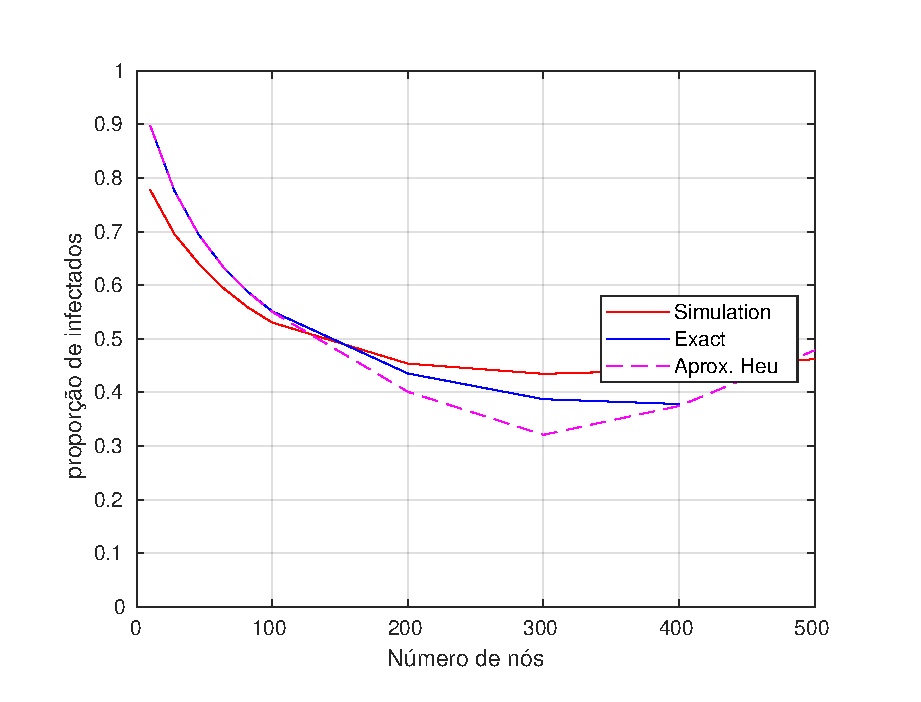
\includegraphics[width=0.35\columnwidth]{img/fig_a_1000_v0_lambda1500_mu17_9593_gamma1_007100_iter_2_rho0_0.pdf} & 
	        \hspace{-0.6cm}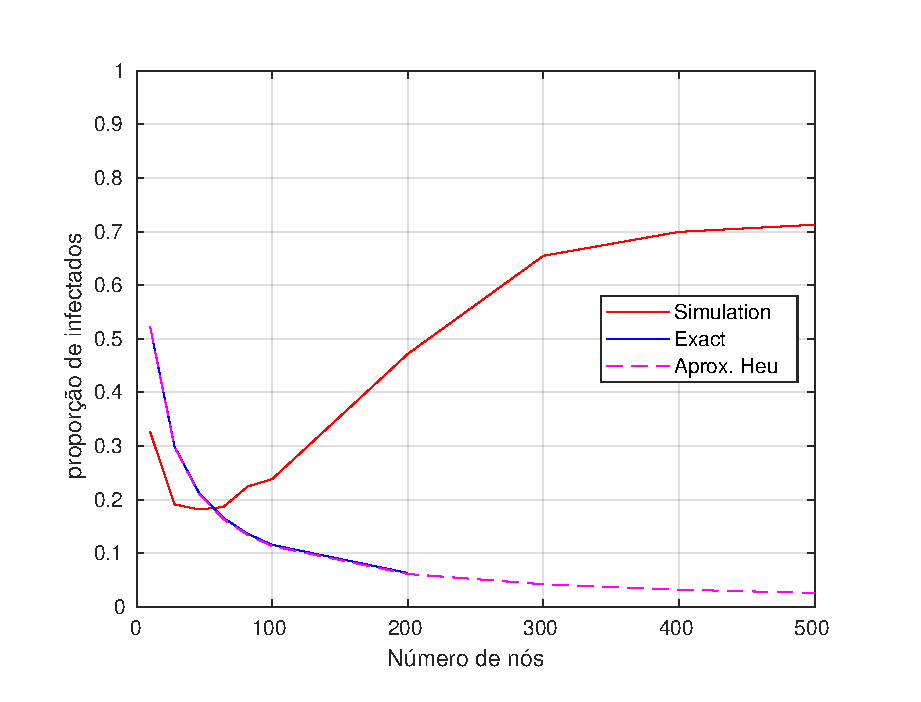
\includegraphics[width=0.35\columnwidth]{img/fig_e_2000_v0_lambda1500_mu154_8883_gamma1_026200_iter_2_rho0_0.pdf} &
	        \hspace{-0.6cm}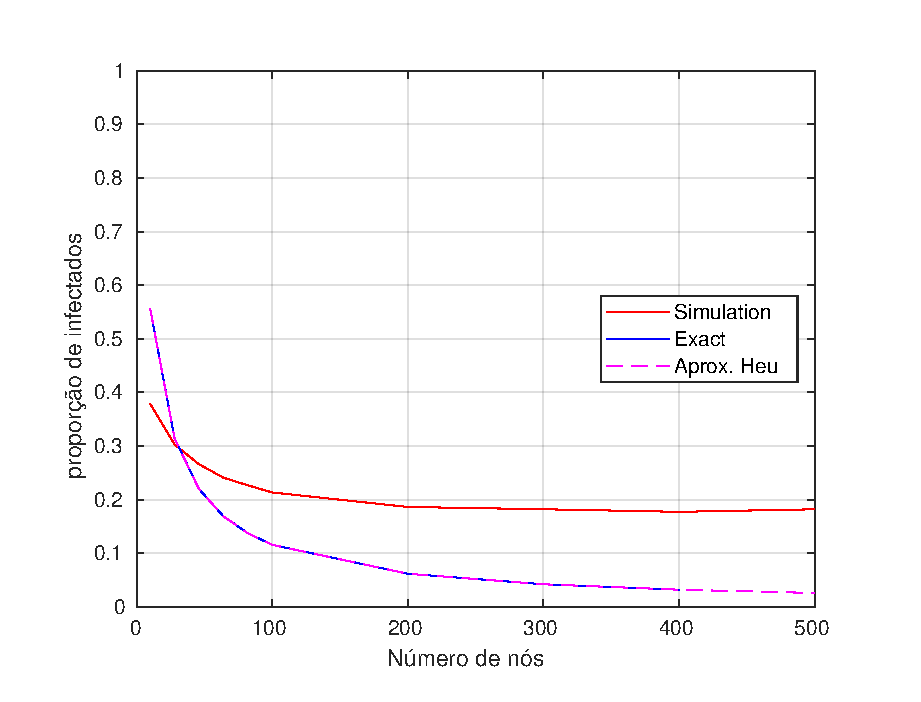
\includegraphics[width=0.35\columnwidth]{img/fig_i_3000_v0_lambda1500_mu122_9877_gamma1_006100_iter_2_rho0_0.pdf}\\
	        (a) $\alpha = 8 \times 10^{-5}$ & 
	        (b) $\beta  = 5 \times 10^{-2}$ & 
	        (c) $\tau   = 18$\\
	        $\mu = 17.959$, $\gamma = 1.0071$ &
            $\mu = 154.888$, $\gamma = 1.0262$ &
            $\mu = 122.987$, $\gamma = 1.0061$\\
	        %------------------------------------------------------
	        \hspace{-0.6cm}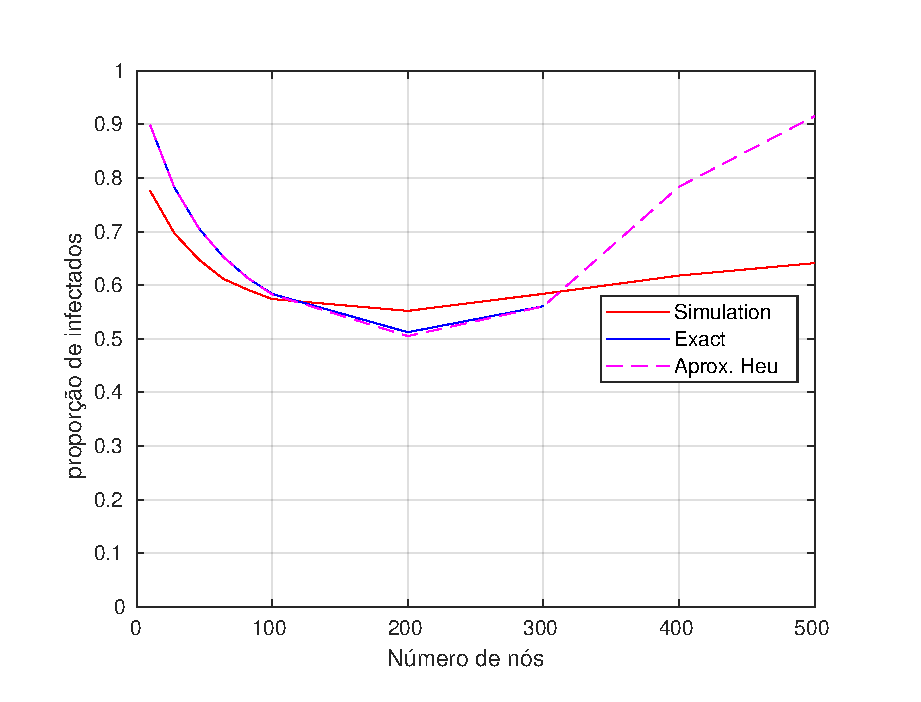
\includegraphics[width=0.35\columnwidth]{img/fig_b_1001_v0_lambda1500_mu18_1603_gamma1_009200_iter_2_rho0_0.pdf} & 
	        \hspace{-0.6cm}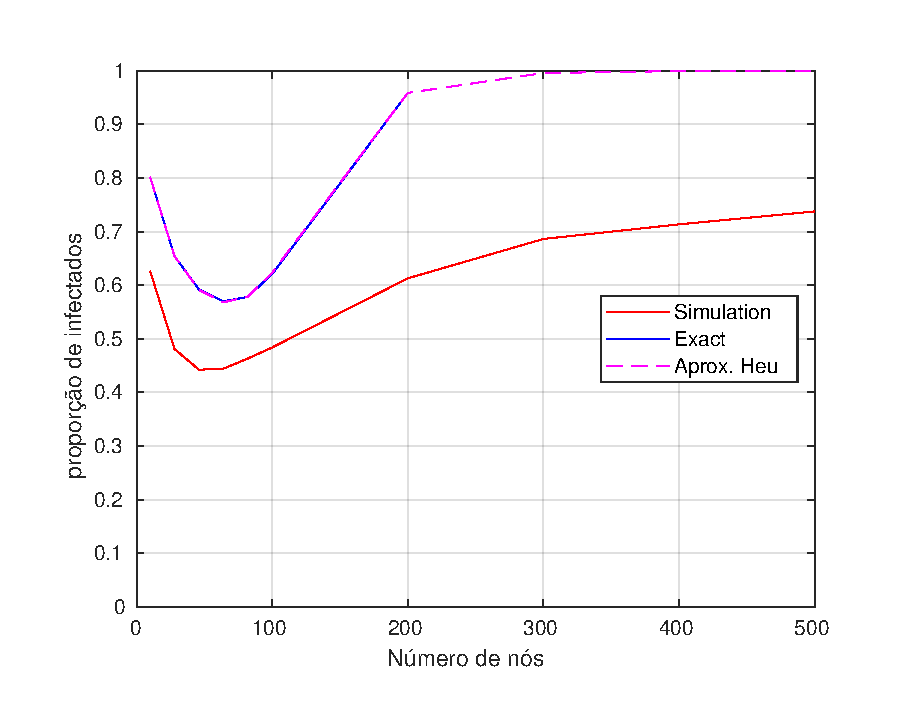
\includegraphics[width=0.35\columnwidth]{img/fig_f_2001_v0_lambda1500_mu44_7099_gamma1_026200_iter_2_rho0_0.pdf} &
	        \hspace{-0.6cm}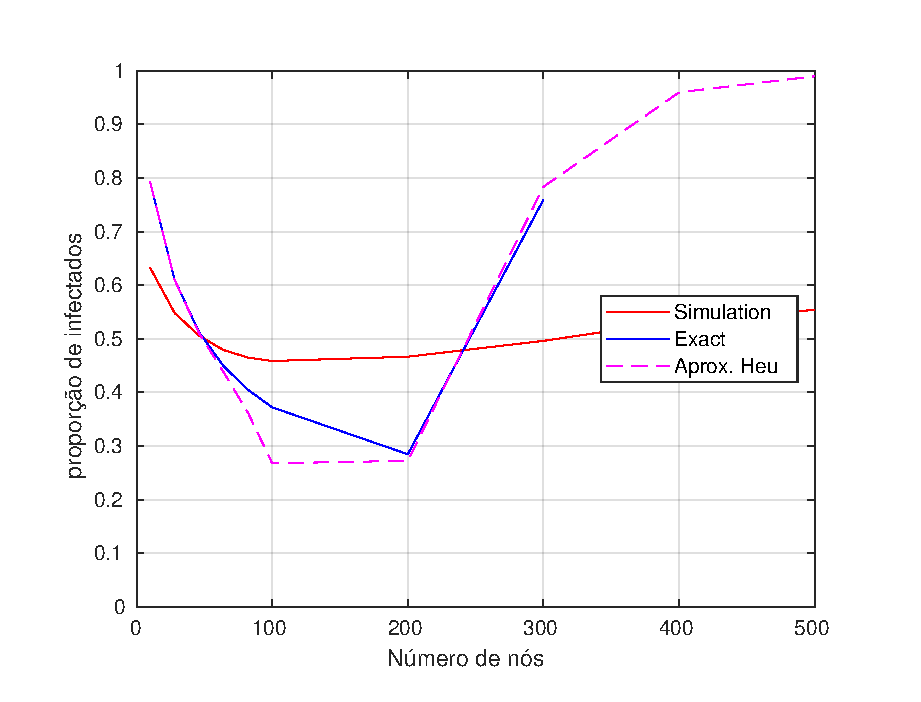
\includegraphics[width=0.35\columnwidth]{img/fig_j_3001_v0_lambda1500_mu43_5209_gamma1_014800_iter_2_rho0_0.pdf}\\
	        (d) $\alpha = 20 \times 10^{-5}$ & 
	        (e) $\beta  = 32 \times 10^{-2}$ & 
	        (f) $\tau   = 40$\\
	        $\mu = 18.160$, $\gamma = 1.0092$ &
            $\mu = 44.710$, $\gamma = 1.0262$ &
            $\mu = 43.521$, $\gamma = 1.0148$ \\
	        %------------------------------------------------------
	        \hspace{-0.6cm}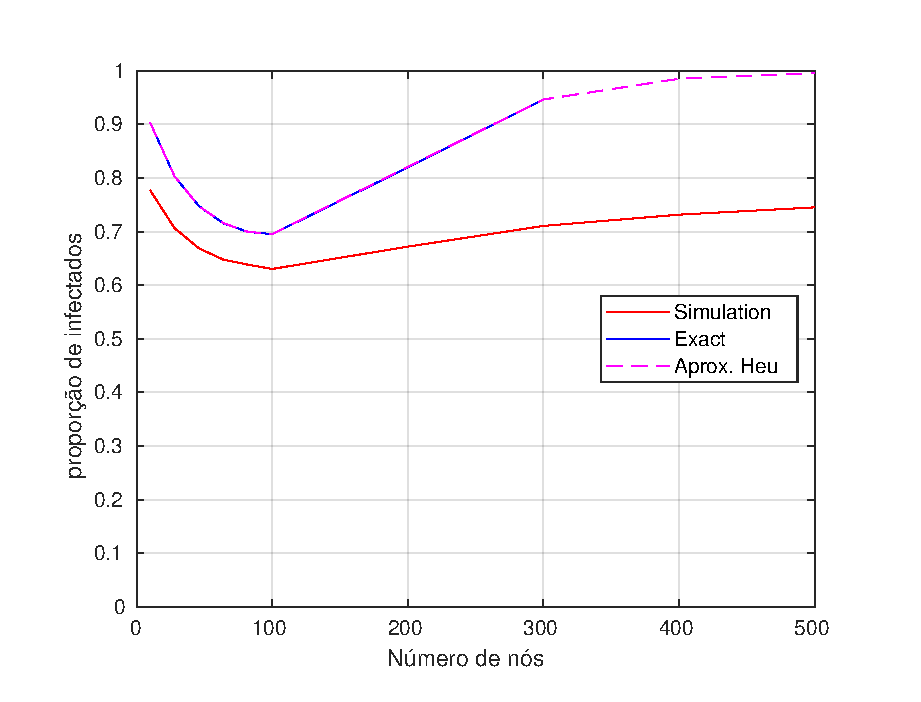
\includegraphics[width=0.35\columnwidth]{img/fig_c_1002_v0_lambda1500_mu18_0462_gamma1_014800_iter_2_rho0_0.pdf} & 
	        \hspace{-0.6cm}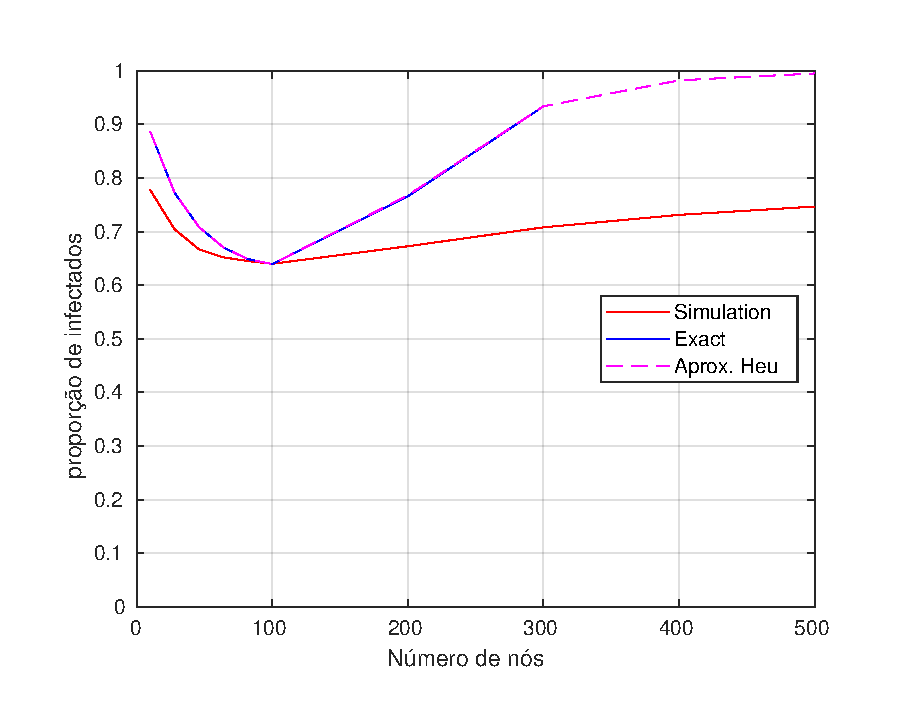
\includegraphics[width=0.35\columnwidth]{img/fig_g_2002_v0_lambda1500_mu21_4111_gamma1_014800_iter_2_rho0_0.pdf} &
	        \hspace{-0.6cm}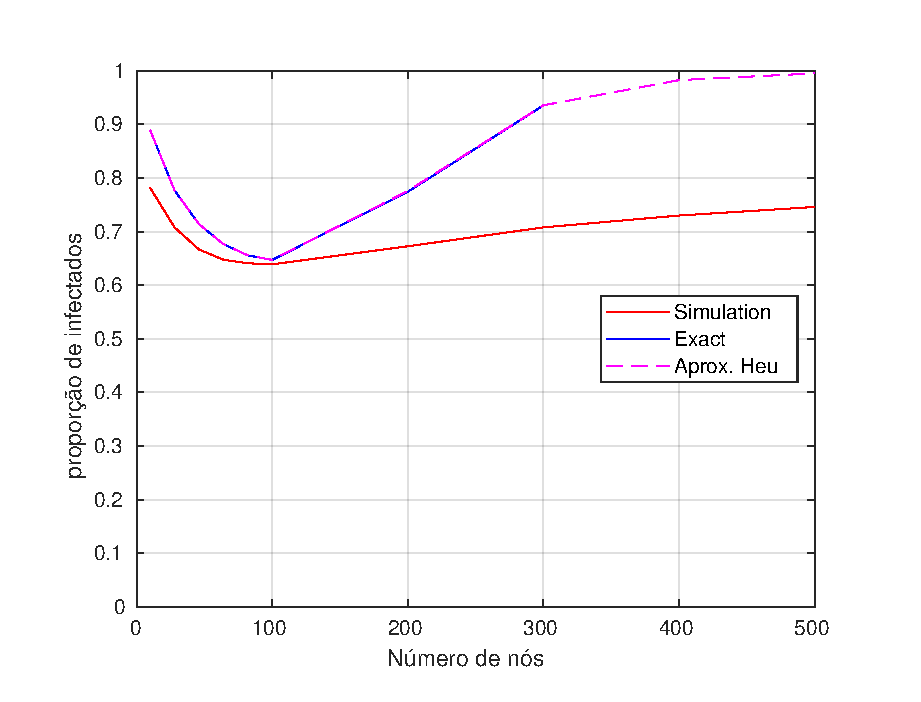
\includegraphics[width=0.35\columnwidth]{img/fig_k_3002_v0_lambda1500_mu20_9333_gamma1_014800_iter_2_rho0_0.pdf}\\
	        (g) $\alpha = 50 \times 10^{-5}$ & 
	        (h) $\beta  = 200 \times 10^{-2}$ & 
	        (i) $\tau   = 65$\\
	        $\mu = 18.046$, $\gamma = 1.0148$ &
            $\mu = 15.717$, $\gamma = 1.0071$ &
            $\mu = 2.882$, $\gamma = 1.0171$ \\
	        %------------------------------------------------------
	        \hspace{-0.6cm}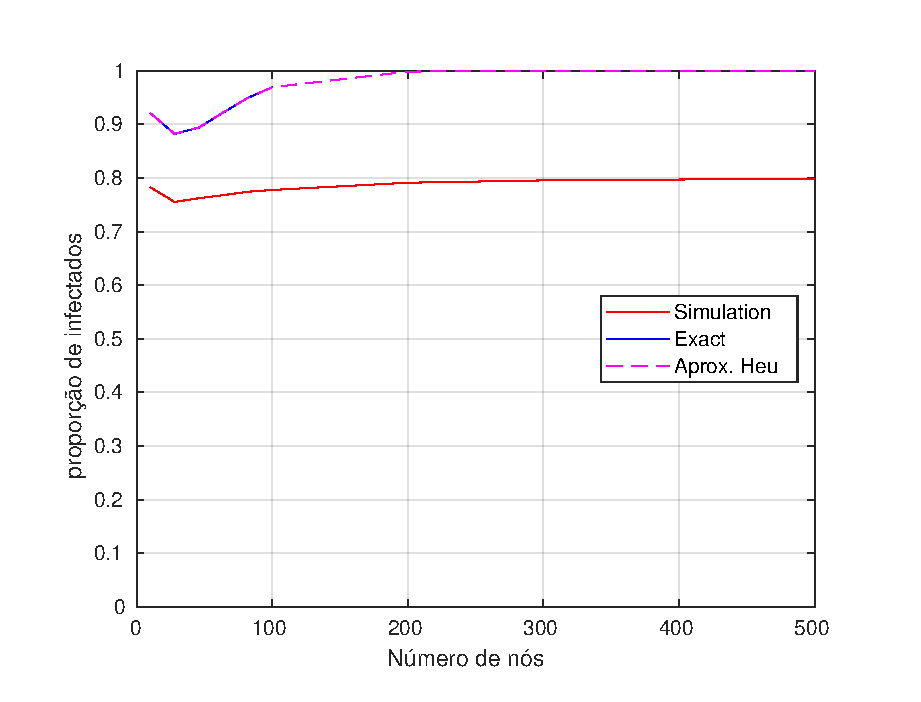
\includegraphics[width=0.35\columnwidth]{img/fig_d_1003_v0_lambda1500_mu17_4592_gamma1_038300_iter_2_rho0_0.pdf} & 
	        \hspace{-0.6cm}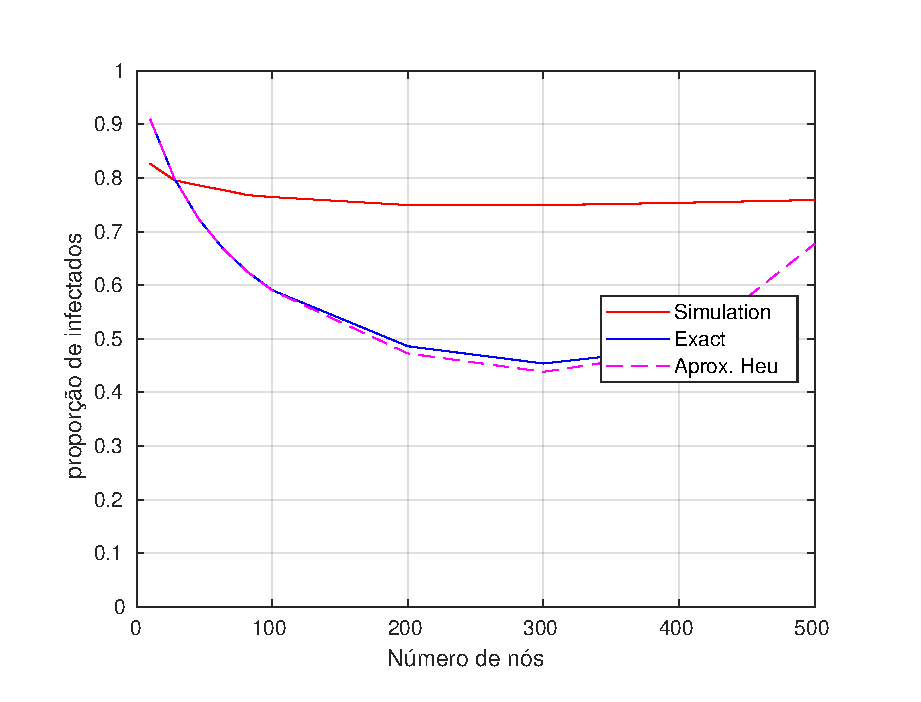
\includegraphics[width=0.35\columnwidth]{img/fig_h_2003_v0_lambda1500_mu15_7172_gamma1_007100_iter_2_rho0_0.pdf} &
	        \hspace{-0.6cm}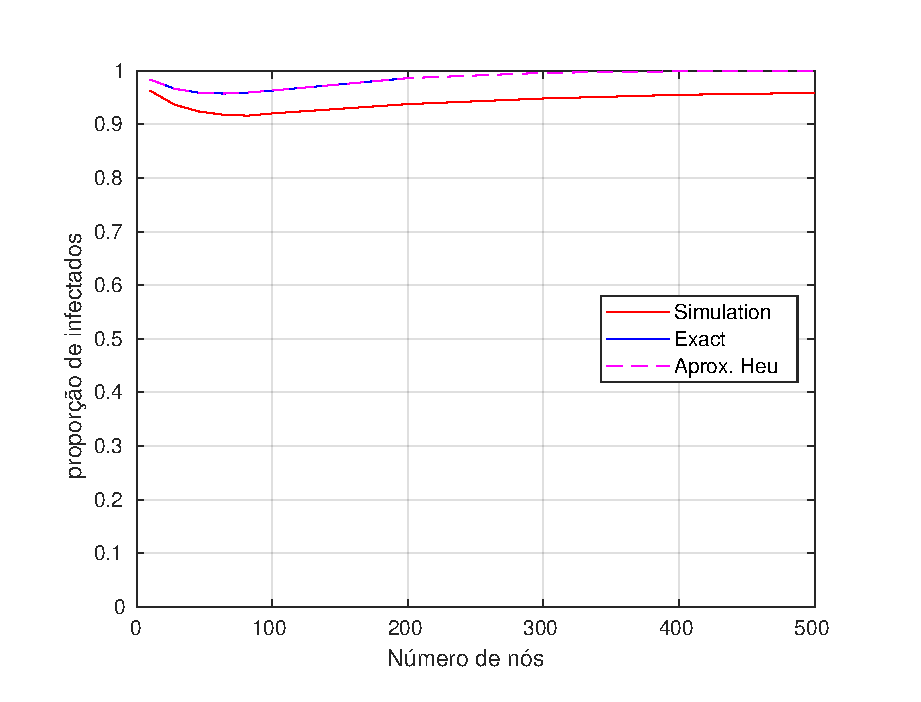
\includegraphics[width=0.35\columnwidth]{img/fig_l_3003_v0_lambda1500_mu2_8819_gamma1_017100_iter_2_rho0_0.pdf}\\
	        (j) $\alpha = 500 \times 10^{-5}$ & 
	        (k) $\beta  = 2000 \times 10^{-2}$ & 
	        (l) $\tau   = 260$ \\
	        $\mu = 17.459$, $\gamma = 1.0383$ &
            $\mu = 21.411$, $\gamma = 1.0148$ &
            $\mu = 20.933$, $\gamma = 1.0148$ 
	        %------------------------------------------------------
	    \end{tabular}
	    \caption{Resultados de simulação para o comportamento da rede totalmente conectada, sob atuação da \textit{Botnet Mirai}  na presença de um atacante estratégico.  Modelo analítico da Seção~\ref{sec:fechadageral} parametrizado com $\Lambda = 1500$ e valores adicionais indicados na figura. }
	    \label{fig:simulacao_resultados_1a_parte}
	\end{figure}
	
	
	
		\textbf{Modelo analítico e simulação}  A Fig.~\ref{fig:simulacao_resultados_1a_parte}  ilustra a probabilidade de infecção segundo o modelo analítico proposto (tanto solução exata quanto  aproximada, nas curvas rosa e azul, respectivamente).   O modelo captura qualitativamente o comportamento da simulação, indicando que no regime inicial, quando o número de nós na rede é pequeno, o sistema é dominado por infecções exógenas.  Na medida em que o número de nós na rede aumenta, a probabilidade de infecção primeiro diminui e depois aumenta, atingindo o segundo regime no qual   o sistema é dominado por infecções endógenas.  
		
	Em geral, o modelo tende a superestimar a probabilidade de infecção em relação à simulação.  Isto deve-se ao fato de que $(i)$ no modelo assumimos que os nós estão sempre ligados, enquanto que na simulação os nós alternam entre ligados e desligados,   $(ii)$  o modelo assume contribuições multiplicativas das taxas de infecção, enquanto que a simulação considera contribuições aditivas e $(iii)$  no modelo, todos os tempos entre eventos são exponencialmente distribuídos, enquanto que na simulação a latência na rede é uniforme (tal latência não é levada em conta no modelo).  Trabalhos futuros consistem em verificar sob que condições o modelo  produz um limite superior para a probabilidade de infecção de fato observada na rede.   Note também que embora a aproximação proposta tenha apresentado bons resultados na Figura~\ref{fig:rho_exact_approx_newton_rho0_0e1}, em alguns cenários da Figura~\ref{fig:simulacao_resultados_1a_parte} a aproximação distanciou-se do valor exato previsto pelo modelo, e estamos no momento averiguando formas de refinar a aproximação.  
	
	    
	    \textbf{Análise de sensitividade} Para estudar a sensitividade da probabilidade de infecção em função dos diferentes parâmetros do sistema, mantemos todos os parâmetros fixos e variamos um de cada vez para avaliar seu impacto.   Em particular, na primeira, segunda e terceira colunas da Figura~\ref{fig:simulacao_resultados_1a_parte} variamos a taxa de contaminação endógena ($\alpha$), taxa de contaminação exógena ($\beta$) e tempo médio que o dispositivo permanece ligado ($\tau$). Nas curvas obtidas via simulação indicamos o intervalo de confiança de $95\%$.   As linhas roxa e verde correspondem, respectivamente, à solução exata do modelo (eq.~\eqref{eq:scaledSISProbIotaInfected}) e à aproximação de Newton, com duas iterações, conforme  heurística definida na Seção~\ref{subsec:heuristica}. 
	     \emph{Cabe ressaltar que o simulador caracteriza detalhadamente o  comportamento do \textit{Mirai Botnet}, enquanto  o modelo proposto  captura a essência do  sistema.}
	    
\emph{O sistema passa por dois regimes fundamentais, primeiro sendo dominado por infecções endógenas e depois por infecções exógenas. }	    Em todos os cenários apresentados na Figura~\ref{fig:simulacao_resultados_1a_parte} observa-se  que o sistema passa por dois regimes.  Tal fato pode ser constatado focando-se nas linhas pontilhadas e tracejadas, que crescem e diminuem, respectivamente,  na medida em que o número de nós no sistema aumenta.   Tal comportamento observado em simulações está de acordo com o previsto pelas equações~\eqref{eq:mainlema1} e \eqref{eq:newton_general}.  No primeiro regime, o sistema é dominado por infecções exógenas (linha tracejada  acima da linha pontilhada).  Na medida em que o número de nós na rede aumenta, as infecções endógenas também passam a exercer papel  importante.  No segundo regime, o sistema é dominado por infecções endógenas (linha tracejada  acima da linha pontilhada).  Em nossas simulações, observamos que o número de nós no sistema correspondente ao cruzamento dos gráficos de infecções endógenas e exógenas (cruzamento das curvas pontilhada e tracejada) é igual ou aproximadamente igual  a aquele que minimiza a  proporção de nós infectados (curva vermelha).
	    
	    
	    
\emph{A probabilidade de infecção é mais sensível à taxa de contaminação endógena  que à taxa de contaminação exógena. } Isto ocorre porque a taxa de infecção endógena é amplificada pelo número de nós infectados na rede, enquanto que a taxa de infecção exógena é limitada pelo \emph{Botmaster}.  Um aumento em torno de $60$ vezes da taxa de infecção endógena produz os efeitos observados na primeira coluna da Figura~\ref{fig:simulacao_resultados_1a_parte}.  Já  a taxa de infecção exógena teve um aumento de $400$ vezes para observarmos a variação de  padrões na segunda coluna da  Figura~\ref{fig:simulacao_resultados_1a_parte}.
	    

	    
	    \emph{O tempo médio que um dispositivo não vacinado permanece ligado (logo, suscetível) é também um fator relevante na simulação.} O valor  assintótico da fração de nós infectados, por exemplo, depende do tempo médio que um dispositivo permanece ligado, conforme vemos na última coluna da Figura~\ref{fig:simulacao_resultados_1a_parte}.   Na medida em que os nós permanecem mais tempo ligados, a proporção de nós infectados também aumenta. \emph{ Simplesmente desligar os sistemas pode ser uma estratégia eficaz para conter epidemias. Entretanto, tal estratégia pode acabar por atender aos anseios do atacante, de causar um ataque de DDoS por indisponibilidade dos sistemas alvos.}
	    
